\documentclass[11pt, a4paper]{report}
\usepackage[utf8]{inputenc}
\usepackage{pgfplots}

\usepackage[top=2cm, bottom=2.3cm, left=2cm, right=2cm]{geometry}

\title{Graficos das geracoes do NSGA2}
\author{Douglas Nunes de Oliveira}
\date{November 2021}


\begin{document}
    \begin{center}
        \textbf{Utilizando o NSGA2 para o problema DTLZ2.}
        
        \textbf{Gráficos do espaço dos objetivos nas gerações ``1, 20, 40, 60, 80 e 100''}
        
        
    \end{center}
    

    \begin{center}
    \textbf{Geração 1}
\end{center}

\begin{figure}[h]
    \centering
    \label{fig:geracao01}
    
    \begin{tabular}{rl}
        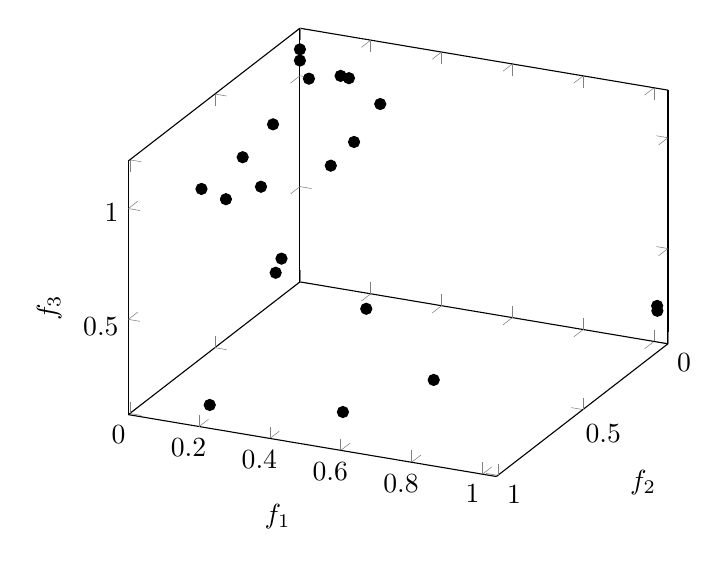
\begin{tikzpicture}[scale=1.0]
        	\begin{axis}[xlabel=$f_2$, ylabel=$f_1$, zlabel=$f_3$, view/h=115]
    			
    			\addplot3[only marks] coordinates {
            		(0.898985, 0.553341, 0.165563) (1.008660, 0.229953, 0.175532) (0.062171, 1.039330, 0.255872) (0.000000, 0.000000, 1.068948) (0.000000, 0.000000, 1.119406) (0.813499, 0.578235, 0.587300) (0.055647, 1.035543, 0.273132) (0.709822, 0.718883, 0.242456) (0.776314, 0.304513, 0.654200) (0.586016, 0.072568, 0.810780) (0.694715, 0.281731, 0.663309) (0.263698, 0.279511, 0.933176) (0.523794, 0.141747, 0.848635) (0.095871, 0.071497, 1.063344) (0.378926, 0.269237, 0.891967) (0.625020, 0.022316, 0.866778) (0.022923, 0.149424, 1.043225) (0.435767, 0.047729, 0.904337) (0.295924, 0.066268, 0.974661) (0.023673, 0.126287, 1.047775) (0.047674, 0.249717, 0.968201) 


        		};
        	\end{axis}
	    \end{tikzpicture}
	    &
	    \begin{tikzpicture}[scale=1.0]
        	\begin{axis}[xlabel=$f_2$, ylabel=$f_1$, zlabel=$f_3$, view={45}{0}]
    			
    			\addplot3[only marks] coordinates {
            		(0.198659,1.402927,0.030436)(0.243016,1.009920,0.490406)(0.965942,0.316067,0.944104)(0.926777,1.057248,0.066572)(0.755361,1.454336,0.018711)(1.099215,0.001117,0.701296)(0.930406,0.386454,0.145874)(0.363359,0.141019,1.073644)(0.005555,0.002258,1.133576)(1.244191,0.475865,0.000000)(0.055722,1.206260,0.087339)(0.122153,0.960673,0.791197)(1.197703,0.000000,0.012183)(0.338440,0.645361,1.002919)(1.231961,0.176431,0.126477)(0.842002,1.466963,0.128832)(1.400163,0.069214,0.140365)(0.050612,0.297072,1.183874)(0.177113,0.032273,1.369730)(0.096804,0.169118,1.443461)(1.185475,0.441860,0.309690) 

        		};
        	\end{axis}
	    \end{tikzpicture}
	\end{tabular}
    
\end{figure}


    \hrulefill
    \begin{center}
    \textbf{Geração 20}
\end{center}

\begin{figure}[h]
    \centering
    \label{fig:geracao01}
    
    \begin{tabular}{rl}
        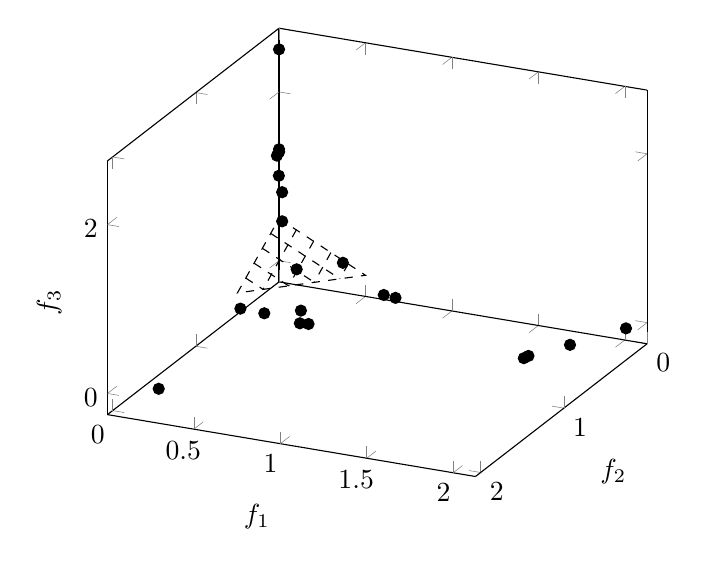
\begin{tikzpicture}[scale=1.0]
        	\begin{axis}[xlabel=$f_2$, ylabel=$f_1$, zlabel=$f_3$, view/h=115]
        		
    			\addplot3[style={dashed}]coordinates {
    			    (0., 0., 0.5) (0., 0.5, 0.) (0.5, 0., 0.) (0., 0., 0.5)
    			};
    			
    			\addplot3[style={dashed}]coordinates {(0., 0.1, 0.4) (0.4, 0.1, 0.)};
    			\addplot3[style={dashed}]coordinates {(0., 0.2, 0.3) (0.3, 0.2, 0.)};
    			\addplot3[style={dashed}]coordinates {(0., 0.3, 0.2) (0.2, 0.3, 0.)};
    			\addplot3[style={dashed}]coordinates {(0., 0.4, 0.1) (0.1, 0.4, 0.)};
    			
    			\addplot3[style={dashed}]coordinates {(0.4, 0., 0.1) (0.4, 0.1, 0.)};
    			\addplot3[style={dashed}]coordinates {(0.3, 0., 0.2) (0.3, 0.2, 0.)};
    			\addplot3[style={dashed}]coordinates {(0.2, 0., 0.3) (0.2, 0.3, 0.)};
    			\addplot3[style={dashed}]coordinates {(0.1, 0., 0.4) (0.1, 0.4, 0.)};
    			
    			\addplot3[only marks] coordinates {
            		(0.196283, 0.196542, 0.115822) (0.269935, 0.735743, 0.053505) (0.031118, 0.033150, 0.502100) (0.752572, 0.276971, 0.046618) (0.003142, 0.002071, 1.292353) (0.280071, 0.808486, 0.052340) (0.589592, 0.410344, 0.000000) (0.806199, 0.164489, 0.103897) (0.000000, 0.000000, 1.320581) (0.008603, 0.003156, 1.014277) (0.753674, 0.483285, 0.000000) (0.253436, 2.128926, 0.125329) (2.062402, 0.296612, 0.157661) (0.000000, 0.000000, 2.503756) (0.732450, 1.768525, 0.013297) (0.745924, 0.529591, 0.001966) (0.046693, 0.010191, 1.284135) (0.253247, 0.491248, 0.337914) (0.613106, 1.978224, 0.152563) (0.101142, 0.066559, 0.911879) (0.712078, 1.785529, 0.030495) 

        		};
        	\end{axis}
	    \end{tikzpicture}
	    &
	    \begin{tikzpicture}[scale=1.0]
        	\begin{axis}[xlabel=$f_2$, ylabel=$f_1$, zlabel=$f_3$, view={45}{0}]
        		
    			\addplot3[style={dashed}]coordinates {
    			    (0., 0., 0.5) (0., 0.5, 0.) (0.5, 0., 0.) (0., 0., 0.5)
    			};
    			
    			\addplot3[only marks] coordinates {
            		(0.000000,0.000000,87.300037)(4.840861,33.459786,20.638485)(48.422177,0.000000,9.858856)(13.120383,31.549160,8.622943)(26.342093,16.373493,6.107313)(0.000000,52.412139,0.000000)(15.055247,28.814203,0.000000)(47.918982,0.001228,9.892156)(51.849355,0.000000,0.000000)(0.000000,0.000000,129.032158)(7.270213,37.696192,24.202731)(44.114677,27.665288,37.262087)(0.000000,92.055748,0.000000)(18.624360,39.312601,2.697538)(53.270066,0.236501,0.000000)(54.632352,0.000000,0.000000)(52.023415,34.357004,0.000000)(159.417210,0.000000,0.000000)(0.000000,168.581518,0.000000)(0.000000,0.000000,130.023145)(60.085897,28.951911,46.264353)

        		};
        	\end{axis}
	    \end{tikzpicture}
	\end{tabular}
    
\end{figure}



    \newpage

    \begin{center}
    \textbf{Geração 40}
\end{center}

\begin{figure}[h]
    \centering
    \label{fig:geracao01}
    
    \begin{tabular}{rl}
        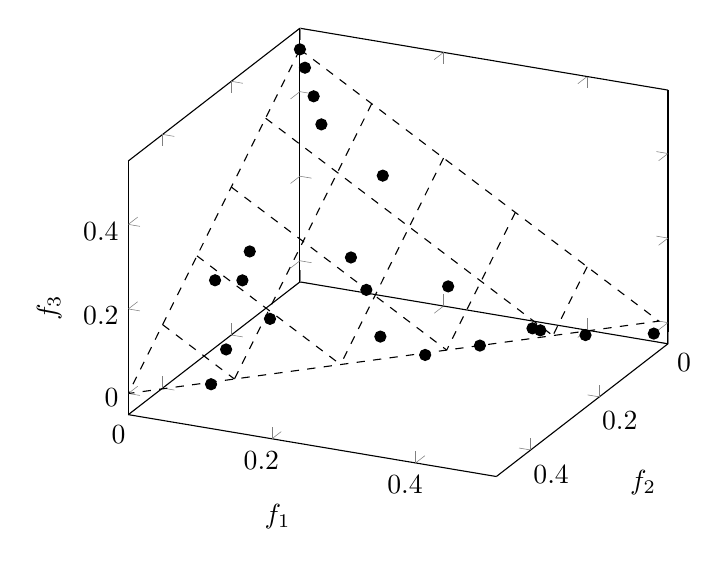
\begin{tikzpicture}[scale=1.0]
        	\begin{axis}[xlabel=$f_2$, ylabel=$f_1$, zlabel=$f_3$, view/h=115]
        		
    			\addplot3[style={dashed}]coordinates {
    			    (0., 0., 0.5) (0., 0.5, 0.) (0.5, 0., 0.) (0., 0., 0.5)
    			};
    			
    			\addplot3[style={dashed}]coordinates {(0., 0.1, 0.4) (0.4, 0.1, 0.)};
    			\addplot3[style={dashed}]coordinates {(0., 0.2, 0.3) (0.3, 0.2, 0.)};
    			\addplot3[style={dashed}]coordinates {(0., 0.3, 0.2) (0.2, 0.3, 0.)};
    			\addplot3[style={dashed}]coordinates {(0., 0.4, 0.1) (0.1, 0.4, 0.)};
    			
    			\addplot3[style={dashed}]coordinates {(0.4, 0., 0.1) (0.4, 0.1, 0.)};
    			\addplot3[style={dashed}]coordinates {(0.3, 0., 0.2) (0.3, 0.2, 0.)};
    			\addplot3[style={dashed}]coordinates {(0.2, 0., 0.3) (0.2, 0.3, 0.)};
    			\addplot3[style={dashed}]coordinates {(0.1, 0., 0.4) (0.1, 0.4, 0.)};
    			
    			\addplot3[only marks] coordinates {
            		(0.428288, 0.080941, 0.000000) (0.041263, 0.512540, 0.000000) (0.000000, 0.000000, 0.500009) (0.067053, 0.147415, 0.285542) (0.065609, 0.061250, 0.381260) (0.257515, 0.053205, 0.198934) (0.378801, 0.078274, 0.050444) (0.042103, 0.039232, 0.426614) (0.311309, 0.030621, 0.158079) (0.309301, 0.106191, 0.087100) (0.108805, 0.386742, 0.014184) (0.242265, 0.227819, 0.037836) (0.184194, 0.159093, 0.168868) (0.293943, 0.060378, 0.155428) (0.109871, 0.376370, 0.016635) (0.168786, 0.331308, 0.000000) (0.081408, 0.436599, 0.000000) (0.015389, 0.014355, 0.470416) (0.226279, 0.282536, 0.000000) (0.204108, 0.190071, 0.113576) (0.136651, 0.271746, 0.102789) 

        		};
        	\end{axis}
	    \end{tikzpicture}
	    &
	    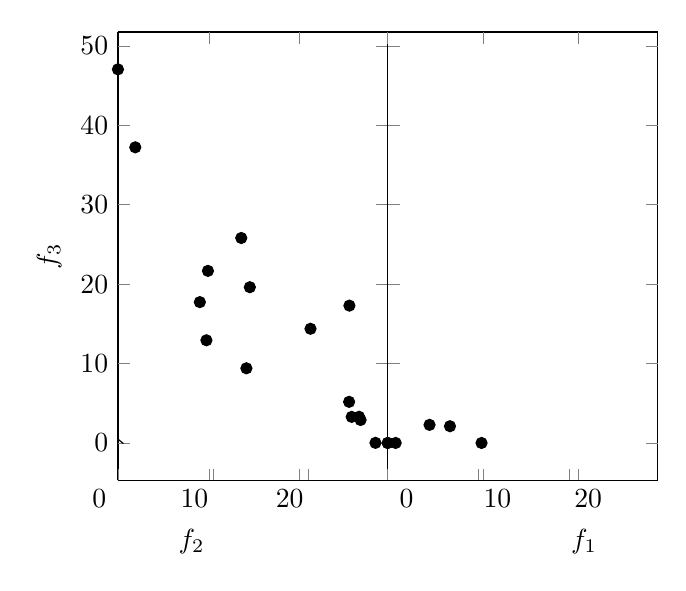
\begin{tikzpicture}[scale=1.0]
        	\begin{axis}[xlabel=$f_2$, ylabel=$f_1$, zlabel=$f_3$, view={45}{0}]
        		
    			\addplot3[style={dashed}]coordinates {
    			    (0., 0., 0.5) (0., 0.5, 0.) (0.5, 0., 0.) (0., 0., 0.5)
    			};
    			
    			\addplot3[only marks] coordinates {
            		(28.347311,0.000000,0.000000)(0.000000,29.690149,0.000000)(0.000000,0.000000,47.036300)(0.007306,1.900215,37.221127)(3.916341,21.368687,17.289221)(5.637196,3.829305,12.926649)(12.955070,0.000000,25.804676)(21.158930,14.373445,2.107765)(9.893921,3.772449,9.401196)(19.927273,13.415639,2.278883)(26.720012,0.349823,0.014184)(8.145637,16.904257,5.176290)(8.017780,1.505578,21.663716)(0.000000,9.011054,17.732197)(1.237240,29.261460,0.000000)(5.018292,15.933057,14.376255)(15.461941,10.337735,3.295152)(13.405901,25.969405,0.000000)(15.840474,10.108729,2.892645)(11.696725,2.261560,19.607841)(0.562518,25.132718,3.284141) 

        		};
        	\end{axis}
	    \end{tikzpicture}
	\end{tabular}
    
\end{figure}


    \hrulefill
    \begin{center}
    \textbf{Geração 60}
\end{center}

\begin{figure}[h]
    \centering
    \label{fig:geracao01}
    
    \begin{tabular}{rl}
        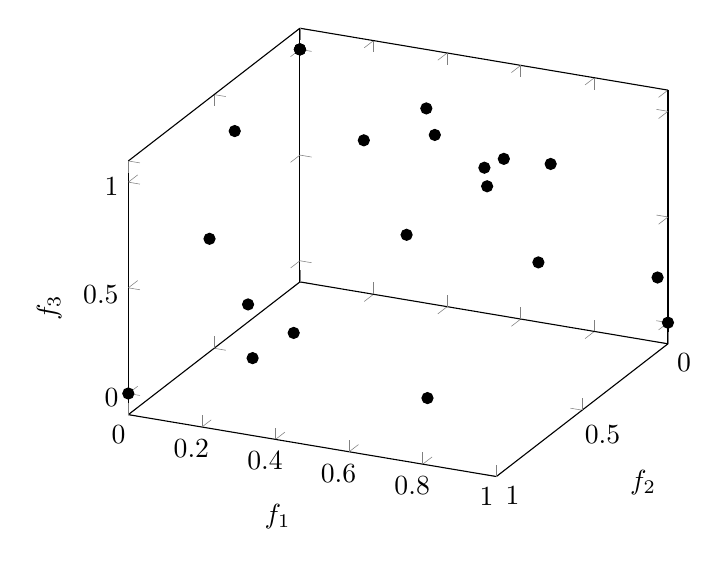
\begin{tikzpicture}[scale=1.0]
        	\begin{axis}[xlabel=$f_2$, ylabel=$f_1$, zlabel=$f_3$, view/h=115]
    			\addplot3[only marks] coordinates {
            		(1.000000, 0.000000, 0.000000) (0.000000, 1.000000, 0.000000) (0.000000, 0.000000, 1.000000) (0.000000, 0.000000, 1.000000) (0.000000, 0.000000, 1.000259) (0.551796, 0.547129, 0.629595) (0.358015, 0.814919, 0.455789) (0.727672, 0.685877, 0.008185) (0.059179, 0.708892, 0.702830) (0.209197, 0.464046, 0.862650) (0.773531, 0.115014, 0.623390) (0.280492, 0.639441, 0.715849) (0.155741, 0.626675, 0.763564) (0.867863, 0.387725, 0.317207) (0.118136, 0.398530, 0.911773) (0.227630, 0.607342, 0.761132) (0.869579, 0.264548, 0.416977) (0.439530, 0.027811, 0.897933) (0.339590, 0.331923, 0.880375) (0.928694, 0.304477, 0.211811) (0.010864, 0.976843, 0.213681) 

        		};
        	\end{axis}
	    \end{tikzpicture}
	    &
	    \begin{tikzpicture}[scale=1.0]
        	\begin{axis}[xlabel=$f_2$, ylabel=$f_1$, zlabel=$f_3$, view={45}{0}]
    			\addplot3[only marks] coordinates {
            		(1.010984,0.000000,0.000000)(0.000000,1.037529,0.000000)(0.000000,0.000000,1.000750)(0.000000,0.000000,1.001416)(0.834344,0.231269,0.523135)(0.708041,0.708917,0.020729)(0.142052,0.333271,0.963492)(0.449248,0.107216,0.891389)(0.514365,0.515286,0.693671)(0.374199,0.827333,0.451951)(0.575647,0.035612,0.818931)(0.431415,0.367960,0.859543)(0.618550,0.586467,0.601420)(0.138000,0.424495,0.920477)(0.591690,0.441873,0.722264)(0.808491,0.024278,0.605166)(0.995947,0.000000,0.178634)(0.983327,0.000000,0.192691)(0.740323,0.551309,0.396134)(0.745135,0.678340,0.241240)(0.247808,0.676069,0.704876) 

        		};
        	\end{axis}
	    \end{tikzpicture}
	\end{tabular}
    
\end{figure}


    
    \newpage
    \begin{center}
    \textbf{Geração 80}
\end{center}

\begin{figure}[h]
    \centering
    \label{fig:geracao01}
    
    \begin{tabular}{rl}
        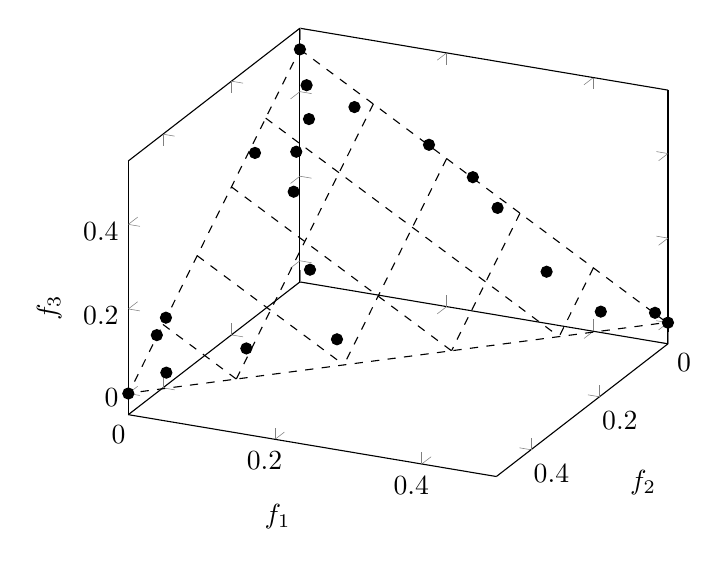
\begin{tikzpicture}[scale=1.0]
        	\begin{axis}[xlabel=$f_2$, ylabel=$f_1$, zlabel=$f_3$, view/h=115]
        		
    			\addplot3[style={dashed}]coordinates {
    			    (0., 0., 0.5) (0., 0.5, 0.) (0.5, 0., 0.) (0., 0., 0.5)
    			};
    			
    			\addplot3[style={dashed}]coordinates {(0., 0.1, 0.4) (0.4, 0.1, 0.)};
    			\addplot3[style={dashed}]coordinates {(0., 0.2, 0.3) (0.3, 0.2, 0.)};
    			\addplot3[style={dashed}]coordinates {(0., 0.3, 0.2) (0.2, 0.3, 0.)};
    			\addplot3[style={dashed}]coordinates {(0., 0.4, 0.1) (0.1, 0.4, 0.)};
    			
    			\addplot3[style={dashed}]coordinates {(0.4, 0., 0.1) (0.4, 0.1, 0.)};
    			\addplot3[style={dashed}]coordinates {(0.3, 0., 0.2) (0.3, 0.2, 0.)};
    			\addplot3[style={dashed}]coordinates {(0.2, 0., 0.3) (0.2, 0.3, 0.)};
    			\addplot3[style={dashed}]coordinates {(0.1, 0., 0.4) (0.1, 0.4, 0.)};
    			
    			\addplot3[only marks] coordinates {
            		(0.501151, 0.000000, 0.000000) (0.000000, 0.501703, 0.000000) (0.000000, 0.000000, 0.500000) (0.041065, 0.355436, 0.103501) (0.000000, 0.235731, 0.266484) (0.156883, 0.064729, 0.280477) (0.359699, 0.094880, 0.045671) (0.013573, 0.275784, 0.214028) (0.000000, 0.175953, 0.325635) (0.040601, 0.429121, 0.030327) (0.066853, 0.043557, 0.389739) (0.279764, 0.181108, 0.042364) (0.449474, 0.027700, 0.025058) (0.112049, 0.047329, 0.341871) (0.145954, 0.006854, 0.348487) (0.018172, 0.082838, 0.399070) (0.226296, 0.119396, 0.155472) (0.417883, 0.000000, 0.085942) (0.391287, 0.000000, 0.110476) (0.035204, 0.025521, 0.444716) (0.000000, 0.484058, 0.018173) 

        		};
        	\end{axis}
	    \end{tikzpicture}
	    &
	    \begin{tikzpicture}[scale=1.0]
        	\begin{axis}[xlabel=$f_2$, ylabel=$f_1$, zlabel=$f_3$, view={45}{0}]
        		
    			\addplot3[style={dashed}]coordinates {
    			    (0., 0., 0.5) (0., 0.5, 0.) (0.5, 0., 0.) (0., 0., 0.5)
    			};
    			
    			\addplot3[only marks] coordinates {
            		(25.557095,0.000000,0.000000)(0.000000,19.177327,0.000000)(0.000000,0.000000,15.470869)(3.037656,6.672029,8.936816)(15.434954,1.229393,10.661216)(5.637196,3.829305,12.926649)(4.844314,10.655167,7.300313)(0.000000,12.296822,5.636917)(5.882303,14.099157,1.845874)(8.940586,8.204036,2.127804)(1.165727,16.318428,2.120988)(17.011234,2.938357,0.984301)(11.845078,11.870279,0.000000)(8.867463,13.563037,3.473916)(8.149641,17.784455,0.449559)(23.541033,1.906498,0.000000)(10.861441,1.290302,7.988342)(19.352375,1.159940,3.186702)(9.307486,0.776347,14.370748)(1.583821,18.413031,0.418250)(21.011899,1.370938,1.268155) 

        		};
        	\end{axis}
	    \end{tikzpicture}
	\end{tabular}
    
\end{figure}


    \hrulefill
    \begin{center}
    \textbf{Geração 100}
\end{center}

\begin{figure}[h]
    \centering
    \label{fig:geracao01}
    
    \begin{tabular}{rl}
        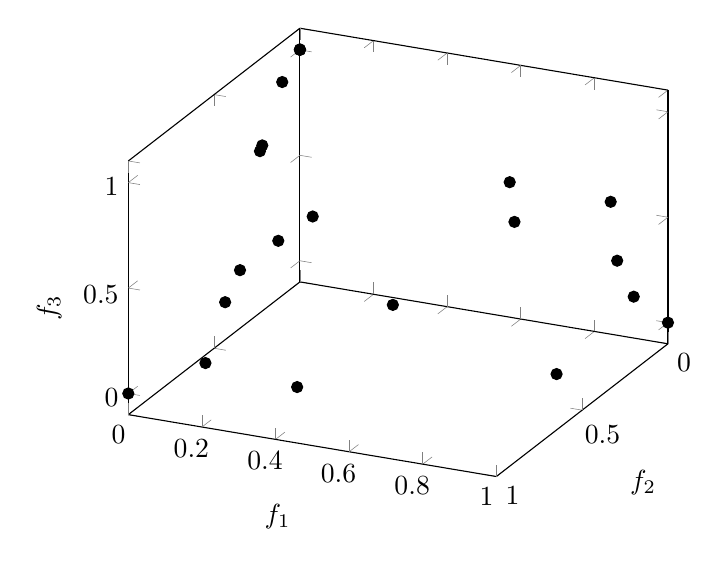
\begin{tikzpicture}[scale=1.0]
        	\begin{axis}[xlabel=$f_2$, ylabel=$f_1$, zlabel=$f_3$, view/h=115]
    			\addplot3[only marks] coordinates {
            		(1.000000, 0.000000, 0.000000) (0.000000, 1.000000, 0.000000) (0.000000, 0.000000, 1.000000) (0.000000, 0.000000, 1.000000) (0.000000, 0.000000, 1.002366) (0.705447, 0.581417, 0.405378) (0.320760, 0.732482, 0.601146) (0.219298, 0.672219, 0.707855) (0.631412, 0.329124, 0.703873) (0.906018, 0.414925, 0.093147) (0.818324, 0.218773, 0.534681) (0.490308, 0.120026, 0.863611) (0.883003, 0.208553, 0.420490) (0.134857, 0.924880, 0.356595) (0.007624, 0.847914, 0.533176) (0.194546, 0.042607, 0.982411) (0.965028, 0.193231, 0.179025) (0.435372, 0.900348, 0.001011) (0.724088, 0.278846, 0.632154) (0.468641, 0.116210, 0.876071) (0.136309, 0.970537, 0.200331) 

        		};
        	\end{axis}
	    \end{tikzpicture}
	    &
	    \begin{tikzpicture}[scale=1.0]
        	\begin{axis}[xlabel=$f_2$, ylabel=$f_1$, zlabel=$f_3$, view={45}{0}]
    			\addplot3[only marks] coordinates {
            		(1.000406,0.000000,0.000000)(0.000000,1.000821,0.000000)(0.000000,0.000000,1.000410)(0.000000,0.000000,1.000513)(0.000000,0.000000,1.008846)(0.428855,0.738966,0.536111)(0.376896,0.857096,0.353981)(0.060711,0.545878,0.837624)(0.577614,0.780391,0.241495)(0.648720,0.240773,0.740718)(0.500330,0.869753,0.178641)(0.771673,0.451443,0.449195)(0.871780,0.307549,0.387998)(0.975467,0.019472,0.228255)(0.027904,0.484476,0.875860)(0.231686,0.510675,0.829175)(0.490248,0.825942,0.289970)(0.828461,0.410978,0.383852)(0.212737,0.088363,0.975027)(0.730887,0.335500,0.608352)(0.483225,0.876988,0.015638) 

        		};
        	\end{axis}
	    \end{tikzpicture}
	\end{tabular}
    
\end{figure}


    
    \newpage
    \begin{center}
    \textbf{Geração 1000}
\end{center}

\begin{figure}[h]
    \centering
    \label{fig:geracaoXX}
    
    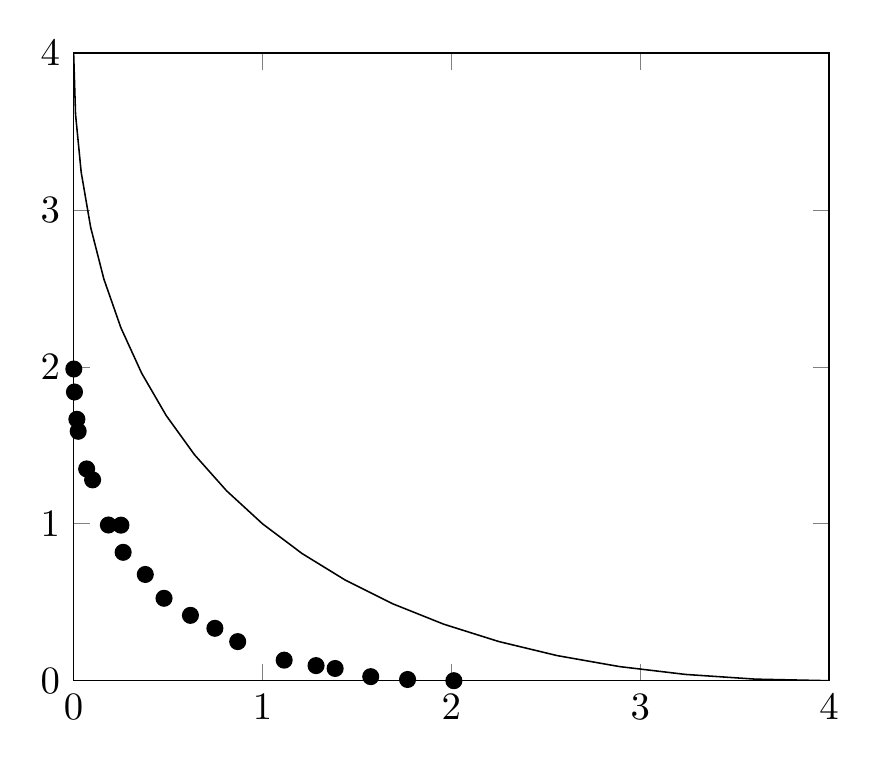
\begin{tikzpicture}[scale=1.4]
        \begin{axis}[enlargelimits=false]
            \addplot [] coordinates {
                (0.000000,4.000000) (0.010000,3.610000) (0.040000,3.240000) (0.090000,2.890000) (0.160000,2.560000) (0.250000,2.250000) (0.360000,1.960000) (0.490000,1.690000) (0.640000,1.440000) (0.810000,1.210000) (1.000000,1.000000) (1.210000,0.810000) (1.440000,0.640000) (1.690000,0.490000) (1.960000,0.360000) (2.250000,0.250000) (2.560000,0.160000) (2.890000,0.090000) (3.240000,0.040000) (3.610000,0.010000) (4.000000,0.000000) 
            };
            
            \addplot [only marks] coordinates {
                (2.013170,0.000022)(0.000811,1.986390)(1.114710,0.131126)(0.379304,0.677108)(0.478528,0.525250)(0.100382,1.280112)(1.767965,0.007815)(1.572890,0.025887)(0.262084,0.818221)(0.183932,0.992356)(0.868628,0.249256)(0.068938,1.349704)(0.024135,1.589631)(1.384435,0.078019)(0.004371,1.839921)(1.283436,0.096246)(0.618352,0.416527)(0.747836,0.333917)(0.017118,1.666182)(0.250461,0.991359) 
            };
        \end{axis}
    \end{tikzpicture}
\end{figure}
    \hrulefill

\end{document}
